\documentclass[tikz,border=12pt]{standalone}
\usepackage[T1]{fontenc}
\usepackage{mathpazo}
\usepackage{amsmath,amssymb}
\usetikzlibrary{arrows.meta, positioning, calc}

\definecolor{stblue}{HTML}{7B97AD}
\definecolor{rwgold}{HTML}{B8995E}
\definecolor{sage}{HTML}{7A9A7E}
\definecolor{dkbrown}{HTML}{3D3530}
\definecolor{wmgray}{HTML}{7B7067}
\definecolor{cream}{HTML}{F9F6F0}
\definecolor{border}{HTML}{D4C9B8}
\definecolor{terracotta}{HTML}{C47A6A}

\begin{document}
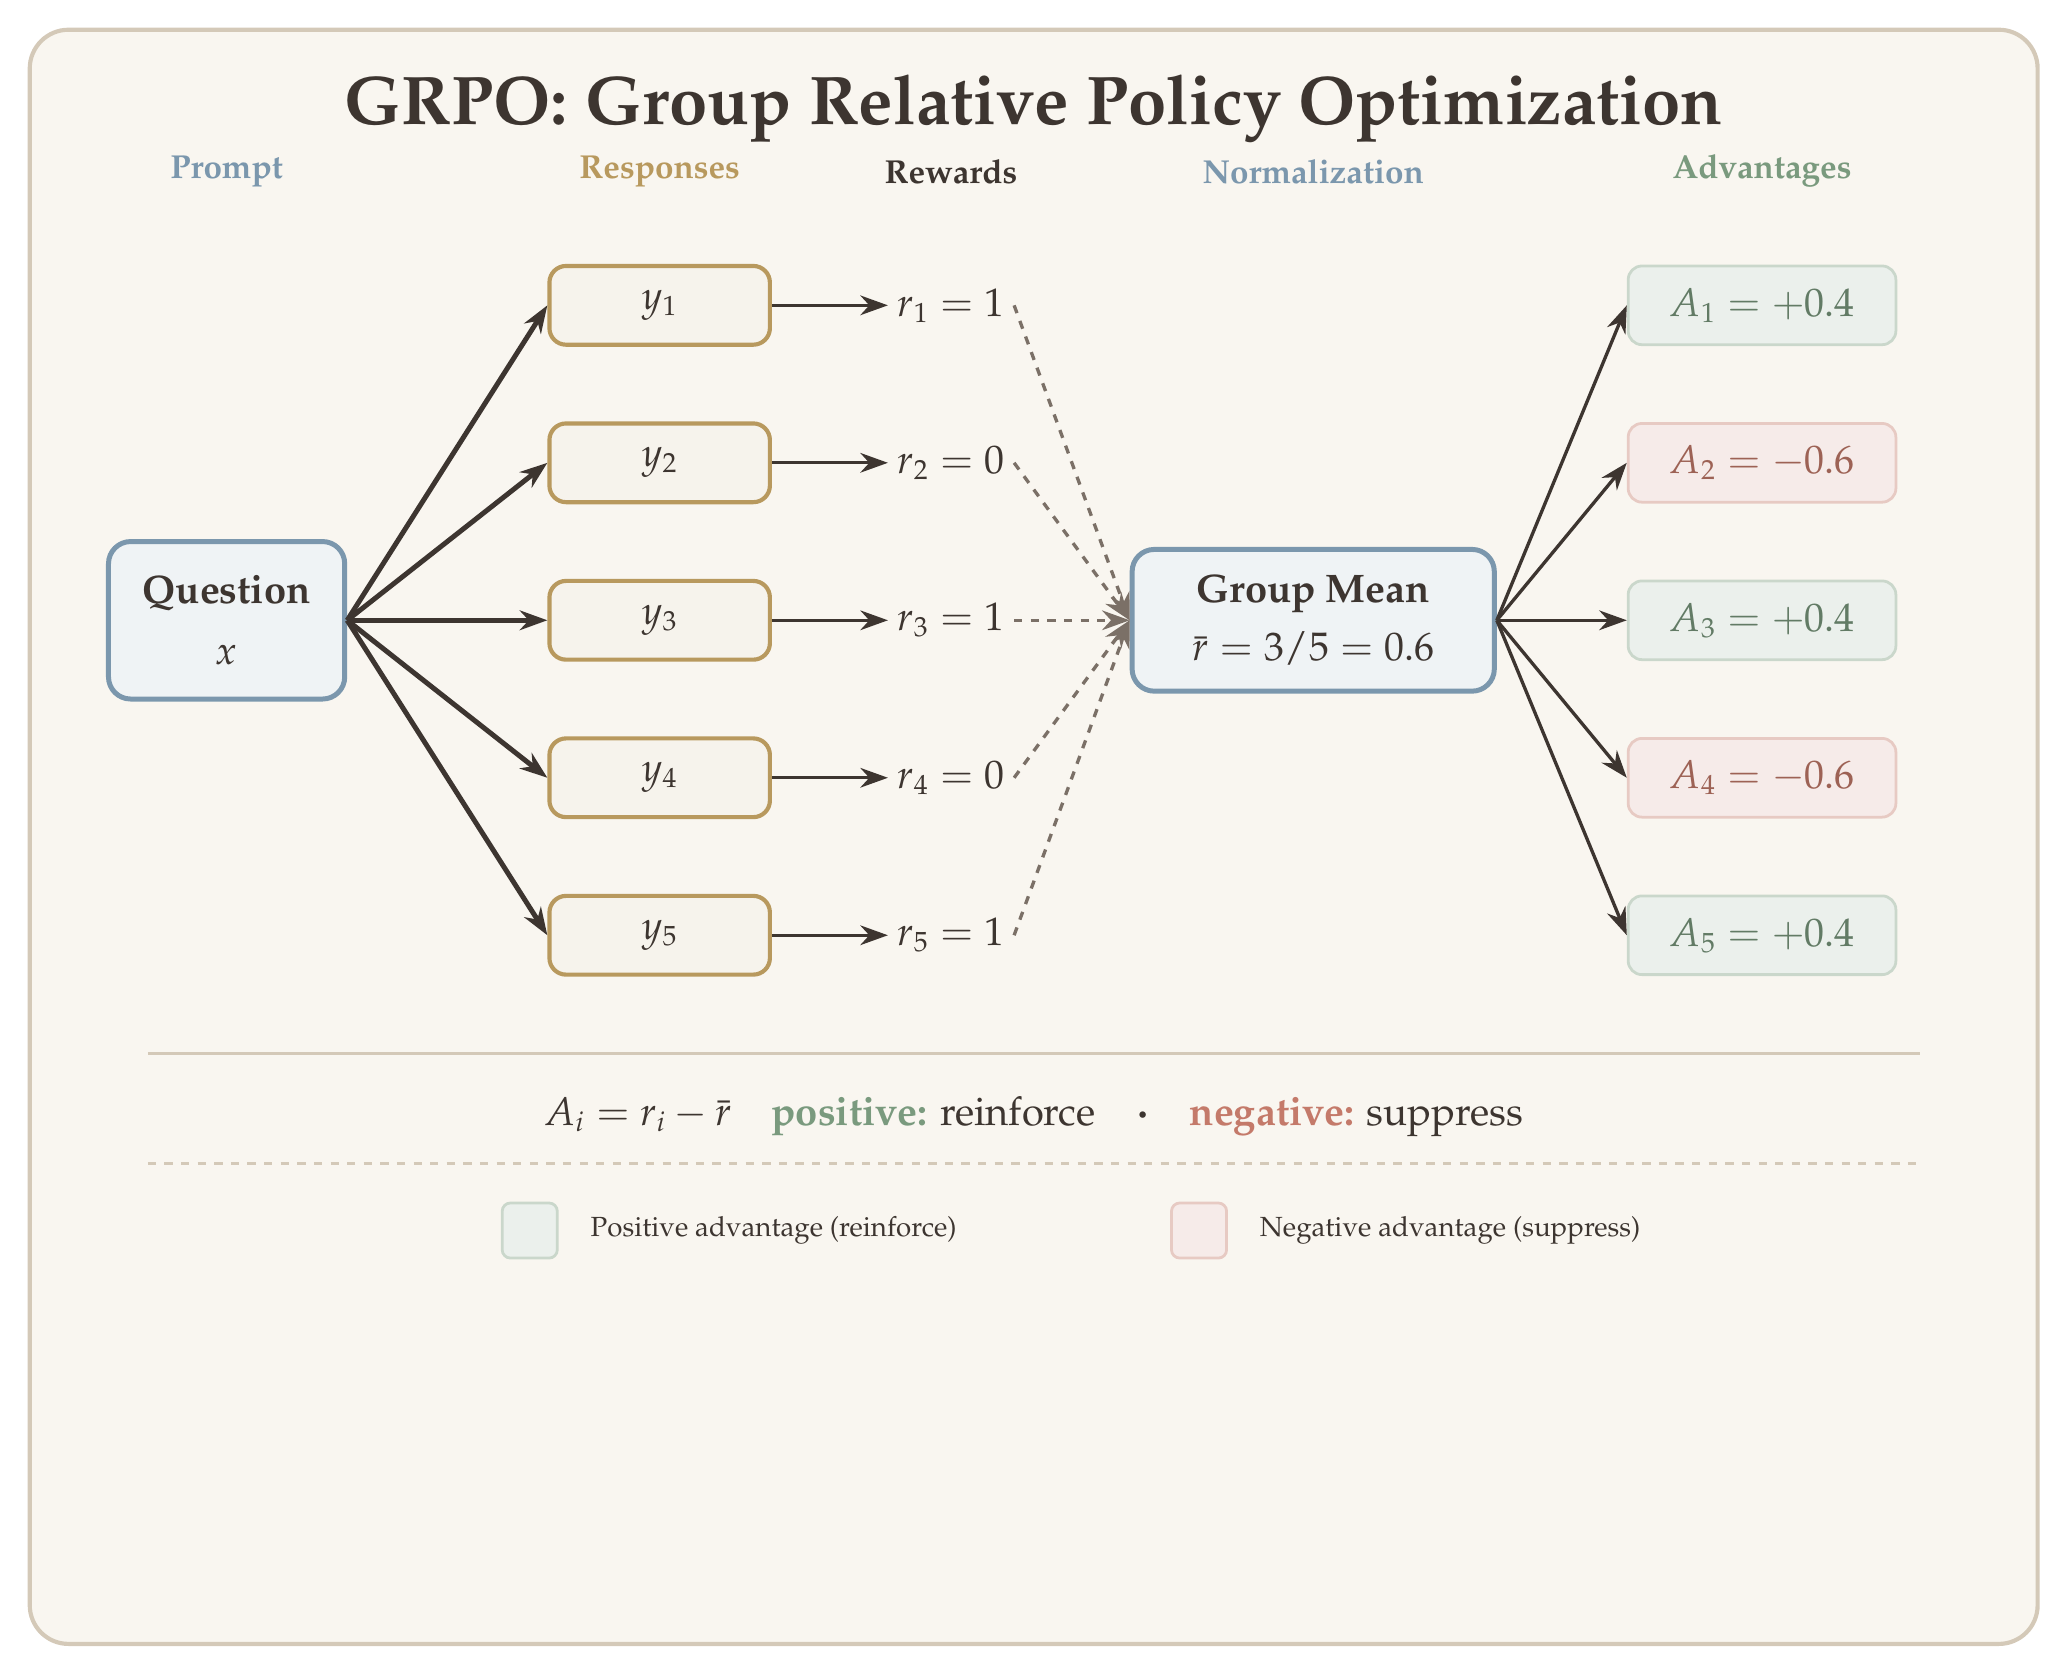
\begin{tikzpicture}[
  >={Stealth[length=3.5mm, width=2.5mm]},
  respbox/.style={
    draw=rwgold, line width=1.5pt, fill=rwgold!12, rounded corners=6pt,
    minimum width=28mm, minimum height=10mm, font=\Large,
    text=dkbrown, align=center, inner sep=5pt
  },
  rewlabel/.style={
    font=\Large, text=dkbrown, align=center
  },
  advbox/.style 2 args={
    draw=#1!40, line width=1pt, fill=#1!15, rounded corners=5pt,
    minimum width=34mm, minimum height=10mm, font=\Large,
    text=#2, align=center, inner sep=4pt
  },
  arr/.style={->, line width=1.8pt, dkbrown},
  darr/.style={->, line width=1.2pt, dashed, wmgray},
  note/.style={font=\normalsize, text=wmgray, align=center},
]

% Background
\fill[cream, rounded corners=14pt] (-1.5,-3.5) rectangle (24,17);
\draw[border, rounded corners=14pt, line width=1.5pt] (-1.5,-3.5) rectangle (24,17);

% Title
\node[font=\Huge\bfseries, text=dkbrown] at (11.25,16)
  {GRPO: Group Relative Policy Optimization};

% ---- Question box ----
\node[draw=stblue, line width=1.8pt, fill=stblue!12, rounded corners=8pt,
  minimum width=30mm, minimum height=20mm, font=\Large,
  text=dkbrown, align=center, inner sep=6pt]
  (question) at (1,9.5)
  {\textbf{Question}\\[4pt] $x$};

% ---- Response boxes ----
\foreach \i/\ypos in {1/13.5, 2/11.5, 3/9.5, 4/7.5, 5/5.5} {
  \node[respbox] (resp\i) at (6.5,\ypos) {$y_{\i}$};
}

% Fan-out arrows from question to responses
\foreach \i in {1,...,5} {
  \draw[arr] (question.east) -- (resp\i.west);
}

% ---- Reward labels ----
\node[rewlabel] (rew1) at (10.2,13.5) {$r_1 = 1$};
\node[rewlabel] (rew2) at (10.2,11.5) {$r_2 = 0$};
\node[rewlabel] (rew3) at (10.2,9.5)  {$r_3 = 1$};
\node[rewlabel] (rew4) at (10.2,7.5)  {$r_4 = 0$};
\node[rewlabel] (rew5) at (10.2,5.5)  {$r_5 = 1$};

% Arrows from responses to rewards
\foreach \i in {1,...,5} {
  \draw[arr, line width=1.2pt] (resp\i.east) -- (rew\i.west);
}

% ---- Group Mean box ----
\node[draw=stblue, line width=1.8pt, fill=stblue!12, rounded corners=8pt,
  minimum width=46mm, minimum height=18mm, font=\Large,
  text=dkbrown, align=center, inner sep=6pt]
  (gmean) at (14.8,9.5)
  {\textbf{Group Mean}\\[3pt] $\bar{r} = 3/5 = 0.6$};

% Dashed lines from rewards to group mean
\foreach \i in {1,...,5} {
  \draw[darr] (rew\i.east) -- (gmean.west);
}

% ---- Advantage boxes ----
\node[advbox={sage}{sage!80!black}]   (adv1) at (20.5,13.5) {$A_1 = +0.4$};
\node[advbox={terracotta}{terracotta!80!black}] (adv2) at (20.5,11.5) {$A_2 = -0.6$};
\node[advbox={sage}{sage!80!black}]   (adv3) at (20.5,9.5)  {$A_3 = +0.4$};
\node[advbox={terracotta}{terracotta!80!black}] (adv4) at (20.5,7.5)  {$A_4 = -0.6$};
\node[advbox={sage}{sage!80!black}]   (adv5) at (20.5,5.5)  {$A_5 = +0.4$};

% Arrows from group mean to advantages
\foreach \i in {1,...,5} {
  \draw[arr, line width=1.2pt] (gmean.east) -- (adv\i.west);
}

% ---- Column headers ----
\node[font=\large\bfseries, text=stblue] at (1,15.2) {Prompt};
\node[font=\large\bfseries, text=rwgold] at (6.5,15.2) {Responses};
\node[font=\large\bfseries, text=dkbrown] at (10.2,15.2) {Rewards};
\node[font=\large\bfseries, text=stblue] at (14.8,15.2) {Normalization};
\node[font=\large\bfseries, text=sage] at (20.5,15.2) {Advantages};

% ---- Bottom formula ----
\node[font=\Large, text=dkbrown] at (11.25,3.2)
  {$A_i = r_i - \bar{r}$\quad
   {\color{sage}\textbf{positive:}} reinforce\quad$\boldsymbol{\cdot}$\quad
   {\color{terracotta}\textbf{negative:}} suppress};

% ---- Legend ----
\fill[sage!15, draw=sage!40, line width=1pt, rounded corners=3pt]
  (4.5,1.4) rectangle (5.2,2.1);
\node[font=\normalsize, text=dkbrown, anchor=west] at (5.5,1.75)
  {Positive advantage (reinforce)};

\fill[terracotta!15, draw=terracotta!40, line width=1pt, rounded corners=3pt]
  (13,1.4) rectangle (13.7,2.1);
\node[font=\normalsize, text=dkbrown, anchor=west] at (14,1.75)
  {Negative advantage (suppress)};

% Divider above formula
\draw[border, line width=1pt] (0,4) -- (22.5,4);

% Divider above legend
\draw[border, line width=0.8pt, dashed] (0,2.6) -- (22.5,2.6);

\end{tikzpicture}
\end{document}
